% ============================================================
% SAVE4223 Final Development Report — LaTeX Source
% Compile with: xelatex report.tex
% ============================================================
\documentclass[12pt, a4paper]{article}

% ---- Packages ----
\usepackage[margin=1in, headheight=14pt]{geometry}
\usepackage{graphicx}
\usepackage{booktabs}
\usepackage{tabularx}
\usepackage{enumitem}
\usepackage{hyperref}
\usepackage{xcolor}
\usepackage{float}
\usepackage{caption}
\usepackage{subcaption}
\usepackage{amsmath}
\usepackage{fancyhdr}
\usepackage{titlesec}
\usepackage{tikz}
\usepackage{fontspec}          % XeLaTeX font support
\usepackage{setspace}
\onehalfspacing

% ---- Hyperref styling ----
\hypersetup{
  colorlinks=true,
  linkcolor=blue!70!black,
  urlcolor=blue!70!black,
  citecolor=blue!70!black,
}

% ---- Header / Footer ----
\pagestyle{fancy}
\fancyhf{}
\fancyhead[L]{\small ISDN 3001 — Final Presentation Report}
\fancyhead[R]{\small SAVE4223}
\fancyfoot[C]{\thepage}
\renewcommand{\headrulewidth}{0.4pt}

% ---- Title ----
\title{%
  \textbf{SAVE4223 — Smart RFID Inventory Cabinet}\\[6pt]
  \large Final Development Report
}
\author{
  He Tianlun \quad Li Tsz Yuk \quad Zhang Yue \quad Zhang Yunxin
}
\date{Spring 2026}

% ============================================================
\begin{document}
\maketitle
\thispagestyle{empty}

\begin{abstract}
The SAVE4223 project delivers a zero-friction, RFID-enabled smart inventory cabinet designed for the HKUST Room~4223 maker space.
The system combines UHF RFID bulk scanning, NFC user authentication, and an offline-first edge-computing architecture to automate tool sign-out and return with zero active effort from the user.
This report details the project vision, user study, system specifications, RF shielding engineering, software architecture, component design, and empirical testing results that validate the prototype for real-world deployment.
\end{abstract}

\newpage
\tableofcontents
\newpage

% ============================================================
\section{Project Vision and Problem Definition}
\label{sec:vision}

In high-traffic maker spaces such as HKUST Room~4223, maintaining an accurate inventory of hundreds of small hand tools represents a significant logistical burden.
Traditional manual sign-out sheets are inherently slow and error-prone, creating a friction-heavy environment that inevitably leads to a breakdown in compliance.
As tools are borrowed and returned dozens of times daily, the administrative overhead of manual tracking fails to scale.
The SAVE4223 project marks a strategic shift toward a \textbf{``zero-friction'' accountability model}, utilizing automated edge-computing and RFID sensing to ensure that every item is tracked the instant a drawer closes---requiring zero active effort from the user.

The system addresses three core operational failures identified in the current lab environment:

\begin{itemize}[nosep]
  \item \textbf{Lost Tools (P-01):} Items left on project desks are frequently forgotten because the lab lacks an automated reminder system for outstanding loans.
  \item \textbf{Volume Tracking (P-02):} The sheer volume of inventory makes paper- or spreadsheet-based tracking a functional impossibility as the system scales.
  \item \textbf{Staff Visibility (P-03):} Lab administrators currently operate in a data vacuum, with no real-time inventory levels or historical usage patterns to inform procurement.
\end{itemize}

Our primary mission is the implementation of a seamless \textbf{``Tap.\ Take.\ Tracked.''} workflow.
This architecture balances the creative freedom required by student researchers with the rigorous administrative control necessary for sustainable laboratory management.

% ============================================================
\section{User Study and Background Research}
\label{sec:userstudy}

The development of SAVE4223 was driven by a ``local-first'' iterative design process.
The system evolved from a Semester~1 prototype---a basic proof-of-concept---to the current industrial-grade architecture.
This transition was dictated by the need to resolve fundamental engineering flaws discovered during initial field tests, ensuring the system could survive the ``knock-and-tolerate'' environment of a professional shop.

\subsection*{Key Findings}

Key takeaways from member interviews, lab-staff consultations, and field tests include:

\begin{itemize}[nosep]
  \item \textbf{Optimal Tech Stack:} The combination of UHF RFID for bulk item tracking and NFC for secure user authentication provides the most seamless hands-off experience.
  \item \textbf{Latency Requirements:} Users demand immediate feedback; Semester~1 testing showed that high latency in processing leads to ``unclosed drawer'' errors.
  \item \textbf{Isolation Standards:} Reliable tracking requires 100\,\% read accuracy inside the volume and 0\,\% ``phantom detections'' outside the enclosure.
\end{itemize}

\subsection*{Lessons from the Semester~1 Prototype}

The Semester~1 prototype utilized plastic drawers which, while easy to assemble, were a failure of isolation.
Because plastic is RF-transparent, waves leaked through the back and sides of the stack, leading to massive interference.
Market research confirmed that while a mass-production route using stock steel cabinets is viable, the prototype route---using aluminium extrusions and composite panels---was necessary to validate our bespoke hardware integration and UI feedback loops.

% ============================================================
\section{Finalized System Specifications and Architecture}
\label{sec:specs}

For a system to be mission-critical in a laboratory setting, it must prioritize a \textbf{``local-first, cloud-synced''} architecture.
This ensures that the cabinet remains fully functional during network outages while maintaining a global ground truth via the cloud.

\subsection{System Specifications}

\begin{table}[H]
\centering
\caption{Physical and mechanical specifications.}
\begin{tabularx}{\textwidth}{lX}
\toprule
\textbf{Parameter} & \textbf{Specification} \\
\midrule
Form \& Dimensions & 620\,$\times$\,522\,$\times$\,850\,mm (height matched to standard workbench) \\
Load Capacity      & 200\,kg total, supported by an industrial aluminium skeletal frame \\
Storage Config.    & Dual drawer depths (120\,mm and 170\,mm) for precision tweezers to heavy power drills \\
Mobility           & Heavy-duty casters for single-person maneuverability \\
\bottomrule
\end{tabularx}
\end{table}

\subsection{Product Architecture \& Hardware Stack}

A Raspberry Pi acts as the central orchestrator, managing edge device logic locally to eliminate the high latency found in cloud-only builds.

\begin{table}[H]
\centering
\caption{Hardware component summary.}
\begin{tabularx}{\textwidth}{llX}
\toprule
\textbf{Component} & \textbf{Technical Spec.} & \textbf{Strategic Purpose} \\
\midrule
Main Controller & Raspberry Pi & Local logic orchestrator; manages auth and cloud sync \\
UHF Reader      & 4-channel, 33\,dBm, EPC Gen2 & Full-volume coverage; high-gain sensing across all drawers \\
Locks           & 4$\times$ Electromagnetic locks & Independent per-drawer permissions and security \\
Sensors         & 4$\times$ IR sensors & Real-time physical closure detection (independent of lock) \\
UI Interface    & Touchscreen + QR Scanner & Bilingual guidance and secure identity verification \\
\bottomrule
\end{tabularx}
\end{table}

% ============================================================
\section{Material Science and Shielding Engineering}
\label{sec:shielding}

The SAVE4223 cabinet design manages a fundamental \textbf{``Core Conflict''}: the external enclosure must serve as a perfect RF shield (Faraday cage), while the internal drawer structures must be RF-transparent to allow for full-volume scanning.

\subsection{The Physics of Shielding}

To prevent ``Slit Active Leaky Wave'' interference, we engineered the enclosure based on \emph{skin depth} ($\delta$) and geometric seam requirements.
The skin depth is determined by the formula:

\begin{equation}
  \delta = \frac{1}{\sqrt{\pi f \mu \sigma}}
\end{equation}

where $f$ is frequency (915\,MHz), $\mu$ is permeability, and $\sigma$ is conductivity.
While the calculated skin depth for aluminium is $\sim 2.8\,\mu$m, effective shielding requires a material thickness several multiples of this; we selected \textbf{0.15\,mm Aluminium Composite Panel (ACP)} to ensure total attenuation.
Furthermore, to prevent wave leakage, all geometric seams were kept at $d < \lambda/30$ ($\approx 1$\,cm) and bridged with conductive tape to maintain galvanic continuity.

\subsection{The Architecture of Compromise}

Materials were categorized into three functional regimes:

\begin{enumerate}[nosep]
  \item \textbf{Structural Frame} (Aluminium T-slot Extrusion): Chosen for its ability to bear 200\,kg loads and provide modular attachment points for accessories.
  \item \textbf{RF Enclosure} (Aluminium Composite Panel): Provides the necessary Faraday shielding while allowing for V-groove folding into a crisp industrial form.
  \item \textbf{Internal Components} (PC Hollow Sunboard \& Plywood): Sunboard provides the RFID transparency and ribbed stiffness required for drawer sides, while Plywood serves as the load-bearing drawer base and the tactile ``safe-touch'' top surface.
\end{enumerate}

% ============================================================
\section{Software Stack and User Experience}
\label{sec:software}

Our software stack (NiceGUI, SQLite, Next.js, Supabase) was selected to provide a high-performance edge UI without the need for a separate API layer for local hardware control.

\begin{table}[H]
\centering
\caption{Software technology stack.}
\begin{tabularx}{\textwidth}{llX}
\toprule
\textbf{Layer} & \textbf{Technology} & \textbf{Rationale} \\
\midrule
Edge UI   & NiceGUI (Python)   & Eliminates separate API layers; runs alongside device logic \\
Edge DB   & SQLite             & Network-resilient local storage for mission-critical reliability \\
App / API & Next.js + Vercel   & Streamlined hosting for the \texttt{save4223.isd-hub.com} portal \\
Cloud     & Supabase           & Managed PostgreSQL and object storage for global visibility \\
\bottomrule
\end{tabularx}
\end{table}

\subsection{State Machine Architecture}

The edge device operates through a deterministic state machine with the following flow:

\[
  \text{LOCKED} \;\rightarrow\; \text{AUTHENTICATING} \;\rightarrow\; \text{UNLOCKED} \;\rightarrow\; \text{SCANNING} \;\rightarrow\; \text{LOCKED}
\]

Each state has a dedicated \texttt{on\_enter} handler.
The cabinet supports dual authentication paths: \textbf{NFC card tap} (offline-capable via local cache) and \textbf{QR sign-in} (requires server).
Failed API calls are queued in SQLite for automatic background retry, ensuring true offline-first operation.

\subsection{The User Journey}

\begin{enumerate}[nosep]
  \item Users register at \texttt{save4223.isd-hub.com} to generate a unique pairing QR code.
  \item At the cabinet, they scan the QR and tap their HKUST student card (NFC) to pair.
  \item Once paired, the user simply taps their card to unlock.
  \item Real-time feedback is provided via the LED strip:
    \begin{itemize}[nosep]
      \item \textcolor{red}{\textbf{Red}} --- Warning: drawer is physically unclosed.
      \item \textcolor{green!60!black}{\textbf{Green}} --- Success: drawer is safely locked and transaction recorded.
      \item \textcolor{blue}{\textbf{Blue}} --- Processing: UHF RFID scanning in progress ($\approx 15$\,s).
    \end{itemize}
  \item The web-based ``Tool Library'' provides administrators with live item counts and historical logs, transforming the previously ``invisible'' inventory into actionable data.
\end{enumerate}

% ============================================================
\section{Component Design and Technical Documentation}
\label{sec:components}

We prioritized \textbf{Design for Manufacturability (DfM)}.
While this prototype uses an extrusion-and-panel method for rapid iteration, the mass-production route will utilize stock steel cabinets.
Steel is an excellent UHF shield, and its higher skin depth requirement ($\sim 0.78$\,mm) is naturally met by standard-gauge industrial steel filing cabinets.

\subsection{Hardware Integration}

\begin{itemize}[nosep]
  \item \textbf{Rear Hardware Bay:} The UHF reader is centrally mounted for balanced cable runs to the antennas. The Raspberry Pi is mounted on the left, with PSUs separated on the right to manage thermal load and electromagnetic interference.
  % Placeholder for a figure showing hardware bay layout
  % \begin{figure}[H]
  %   \centering
  %   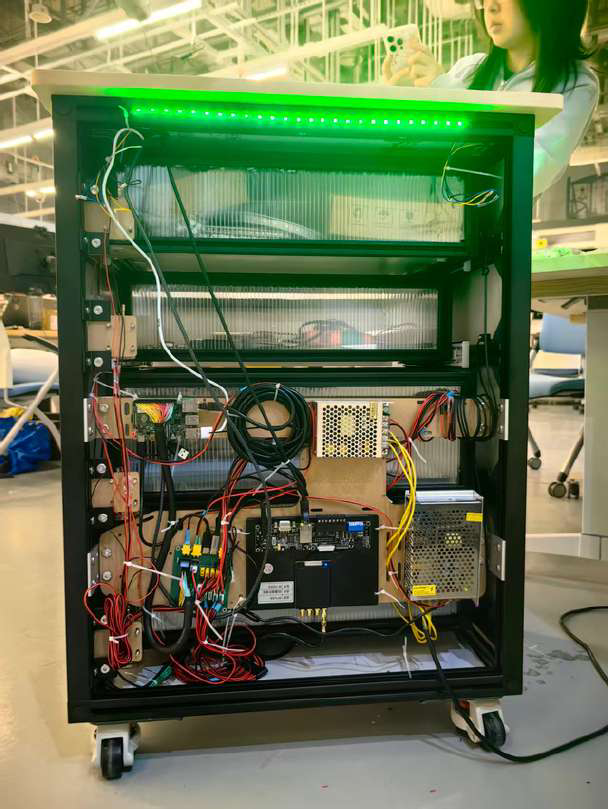
\includegraphics[width=0.8\textwidth]{assets/prototype-internals.png}
  %   \caption{Rear hardware bay layout showing UHF reader, Raspberry Pi, and power supplies.}
  %   \label{fig:hardware-bay}
  % \end{figure}
\end{itemize}

\subsection{Source Code Repositories}

\begin{itemize}[nosep, leftmargin=2em]
  \item \textbf{Edge Device (Raspberry Pi):} \url{https://github.com/year3-project/save4223-cabinet-pi}
  \item \textbf{Cloud Server:} \url{https://github.com/year3-project/save4223server/}
\end{itemize}

\subsection{Project Website}

The final presentation website is published at:

\begin{center}
  \url{https://year3-project.github.io/finalPresentation/}
\end{center}

\subsection{CAD and Fabrication Files}

All CAD models, laser-cut DXF files, and fabrication drawings are available at:

\begin{center}
  \url{https://github.com/year3-project/finalPresentation/tree/cad-files/cad-files}
\end{center}

% ============================================================
\section{Results, Testing, and Performance Evaluation}
\label{sec:results}

Empirical validation was required to ensure survival in a maker-space environment.

\subsection{Mechanical and Surface Testing}

\begin{itemize}[nosep]
  \item \textbf{Three-Point Bending Test:} Confirmed structural integrity under full load.
  \item \textbf{Hardness Evaluation:} We performed Mohs Hardness and ASTM D3363 Pencil Hardness tests. We determined that PC Hollow Sunboard, while excellent for RF transparency, failed the touch-surface test (scratched by a fingernail). Consequently, Sunboard was relegated to internal use, with Plywood used for all touchable surfaces.
\end{itemize}

\subsection{RFID Validation}

The engineering goal was a \textbf{high internal read rate} and \textbf{0\,\% external ``phantom detections.''}
By maintaining a sealed Faraday cage and using conductive tape to bridge galvanic discontinuities, we successfully isolated the 915\,MHz signal.
The hybrid material regime (shielding outer shell / transparent inner drawers) achieved \textbf{high accuracy} in identifying items during the scan cycle.

% ============================================================
\section{Roadmap and Future Improvements}
\label{sec:roadmap}

SAVE4223 is currently a fully functional working prototype, ready for expanded deployment in HKUST Room~4223.

\subsection*{Phased Improvements}

\begin{description}[nosep, style=nextline]
  \item[Short term (3--4 weeks):] Finalize door back-panels, optimize mobile UI data-fetching, and implement concurrency handling for multi-user scenarios.
  \item[Long term (5+ weeks):] Deployment of the full admin platform and the ``Materials System''---a Taobao MCP integration that will auto-generate expense reports and push ordered items directly to inventory.
\end{description}

% ============================================================
\section{Project Team}
\label{sec:team}

\begin{table}[H]
\centering
\begin{tabularx}{\textwidth}{lX}
\toprule
\textbf{Member} & \textbf{Role} \\
\midrule
HE Tianlun (HT)    & Cabinet design lead --- overall cabinet design: mechanical structure and hardware integration \\
LI Tsz Yuk (LT)    & Hardware \& screw cabinet --- tool-cabinet hardware circuit design; screw-cabinet overall design and UI \\
ZHANG Yue (ZY)     & Embedded systems --- embedded software and firmware; screw-cabinet hardware design \\
ZHANG Yunxin (ZY)  & Web platform --- end-to-end website UI design and deployment \\
\bottomrule
\end{tabularx}
\end{table}

% ============================================================
% \section*{References}
% Add any references here using \bibitem or BibTeX.

\end{document}
